\begin{figure}
\centering
\begin{subfigure}[b]{0.3\textwidth}
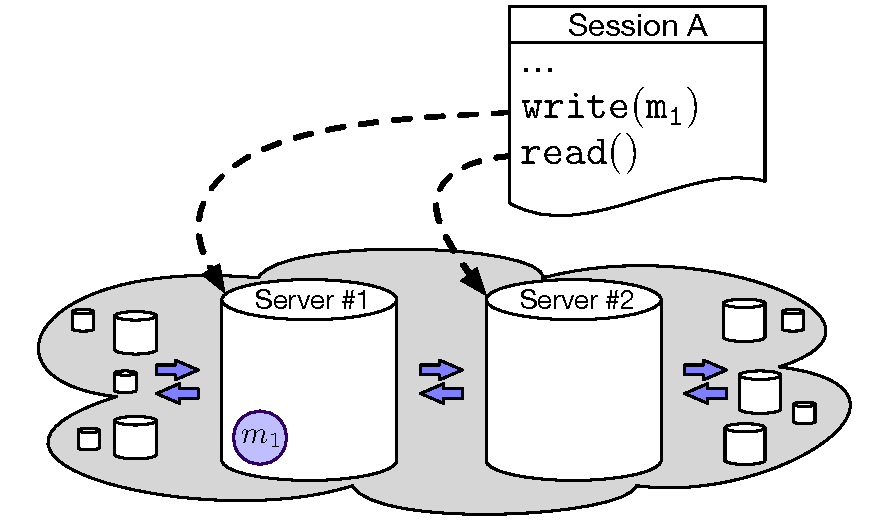
\includegraphics[scale=0.2]{../Figures/System_example.pdf}
\label{fig:rmw_falsified}
\caption{A behavior allowd in EC stores that falsifies RMW guarantee}
\end{subfigure}\quad
\begin{subfigure}[b]{0.3\textwidth}
A figure showing tokens being passed around for enforcing RMW
\label{fig:addhoc_impl}
\caption{An ad-hoc implementation of RMW consistency guarantee, using
tokens and guards}
\end{subfigure}\quad
\begin{subfigure}[b]{0.3\textwidth}
A figure showing how consistency management can be separated from the
applications and underlying stores,using shim layers (our shims are
synthesized according to the given contract)
\label{fig:shim_impl}
\caption{Consistency management shim layer that guarantees desired
levels of consistency, based on the given specifications}
\end{subfigure}~
\caption{Running applications on EC store, ad-hoc consistency
implementations, general-purpose shim layers}



\end{figure}

